\chapter{Fundamentação Teórica}\label{cap:fundamentacao}

Neste capítulo, são apresentados os conceitos e as definições necessárias para o entendimento deste trabalho. A Seção \ref{sec:osteoartrite} apresenta a osteoartrite de joelhos e suas características clínicas. A seção \ref{sec:visao-computacional} aborda a visão computacional na área da saúde. A Seção \ref{sec:aprendizado-profundo} mostra alguns conceitos fundamentais de arquiteturas de aprendizado profundo, incluindo as redes neurais convolucionais e os vision transformers.

% Por fim, a seção \ref{sec:ajuste-fino} apresenta os conceitos de transferência de aprendizado através do ajuste fino de modelos pré-treinados.

\section{Osteoartrite de Joelho}\label{sec:osteoartrite}

\subsection{Definição e Características Clínicas}

A osteoartrite (OA) é definida como uma doença heterogênea e degenerativa, que afeta as articulações e estruturas ósseas de pacientes, causando sintomas de dor, deformidade e perda de função \citep{Loeser2012}. Considerando os fenótipos da doença, ou seja, as características clínicas e radiográficas observáveis, a OA é considerada altamente heterogênea, isso significa que pode ser causada por diversos fatores, incluindo:

\begin{itemize}
    \item \textbf{Idade}: a OA é mais comum em idosos, devido ao desgaste natural e inevitável das articulações ao longo do tempo \citep{ShaneAnderson2010}.
    \item \textbf{Sexo}: mulheres têm maior risco de desenvolver OA do que homens, especialmente após a menopausa, devido à diminuição dos níveis de estrogênio, que protege a cartilagem articular \citep{Tschon2021}.
    \item \textbf{Obesidade}: o excesso de peso também é uma condição de risco para a OA, pois aumenta a carga mecânica nas articulações, influenciando o início e a progressão da doença \citep{PACCA2018}.
    \item \textbf{Predisposição genética}: fatores genéticos também podem influenciar o desenvolvimento da OA, como a presença de mutações em genes relacionados à formação e manutenção da cartilagem articular \citep{Spector2004}.
    \item \textbf{Outros fatores}: lesões articulares, atividade física intensa, doenças metabólicas, entre outros.
\end{itemize}

A OA pode afetar diversas articulações, como joelhos, quadris, mãos, ombros, entre outras. No entanto, a junção do joelho é a área mais afetada devido ao suporte do peso corporal que está diretamente associados a movimentos essenciais, como caminhar, subir escadas e agachar \citep{Kanamoto2020}. Portanto, tais fatores fazem com que a doença seja uma das princiais causas de dor crônica e incapacidade funcional, levando a uma necessidade de identificar e classificar a OA de forma precisa e precoce, para que o tratamento seja iniciado o mais cedo possível a fim de retardar a progressão da doença e melhorar a qualidade de vida dos pacientes.

\subsection{Mudanças Patológicas da OA de Joelhos}

Entre as mudanças patológicas observadas na OA, estão:

\begin{itemize}
    \item \textbf{Degradação da cartilagem articular}: a cartlagem articular é um tecido que reveste as extremidades ósseas, permitindo movimentos suaves e absorção de impactos. Na OA, ocorre uma perda progressiva da matriz cartilaginosa, onde as células da cartilagem, chamadas de condrócitos, se tornam "ativas" e aumentam a produção de enzimas que degradam a matriz \citep{Goldring2009}.
    \item \textbf{Inflamação sinovial}: a membrana sinovial é um tecido que reveste as articulações e produz o líquido sinovial, que lubrifica e nutre a cartilagem. Na OA, ocorre a condição chamada sinovite, onde a membrana sinovial se torna inflamada, causando dano e destruição à cartilagem \citep{Pessler2008}.
    \item \textbf{Degeneração dos ligamentos}: os ligamentos são estruturas que conectam os ossos e estabilizam as articulações. Na OA, os ligamentos podem sofrer rupturas e degeneração, afetando a mecânica articular. Essa degeneração aumenta a predisposição para o desenvolvimento da doença \citep{Loeser2012}.
    \item \textbf{Degeneração do menisco}: o menisco, estrutura fibrocartilaginosa que na absorção de choques e na estabilidade articular, também é afetado na OA. Sua degeneração leva à perda da função de amortecimento e à piora da sobrecarga nas superfícies articulares \citep{Loeser2012}.
    \item \textbf{Alterações ósseas}: o osso subcondral, localizado abaixo da cartilagem, também é afetado na OA, como a formação de osteófitos, que são projeções ósseas anormais, e a esclerose subcondral, que é o aumento da densidade óssea. Essas alterações podem causar dor e limitação de movimentos \citep{vanderKraan2007}.
\end{itemize}

A Figura \ref{fig:osteoartrite-joelho} ilustra as mudanças patológicas observadas na OA de joelhos a partir de imagens de ressonância magnética.

\begin{figure}[h]
    \centering
    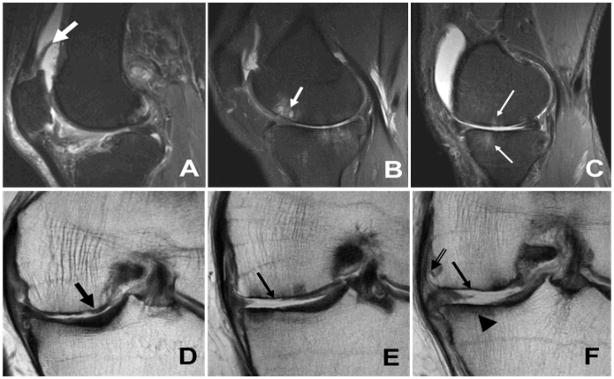
\includegraphics[width=\linewidth]{figs/mud-patologicas-oa.jpg}
    \caption{Imagens de recuperação por inversão sagital (A–C) e eco de spin rápido coronal (D–F) ilustrando os achados da ressonância magnética na osteoartrite. (A) Sinovite reativa (seta branca espessa), (B) Formação de cistos subcondrais (seta branca), (C) Edema da medula óssea (setas brancas finas), (D) Desgaste parcial da cartilagem (seta preta espessa), (E–F) Desgaste total da cartilagem (setas pretas finas), esclerose subcondral (cabeça de seta) e formação de osteófitos marginais (seta dupla). Imagem cortesia dos Drs. Hollis Potter e Catherine Hayter, Hospital for Special Surgery, Nova York, NY. Fonte: \cite{Loeser2012}.}
    \label{fig:osteoartrite-joelho}
\end{figure}

\subsection{Impacto da OA na Qualidade de Vida}

De acordo com o World Health Organization (WHO), "qualidade de vida" é definida como a percepção do indivíduo sobre sua posição de vida no contexto da cultura e sistema de valores que ele vive e em relação aos seus objetivos, expectativas, padrões e preocupações \citep{who2012}.

Existe um grande esforço de pesquisadores e especialistas para avaliar o grau de incapacidade física causado pela doença, além de avaliar os efeitos de diferentes tratamentos em aspectos como dor, função física e mobilidade. No entanto, tais manifestações físicas afetam diretamente outras áreas na vida dos pacientes, como interações sociais, saúde mental e qualidade do sono \citep{Ferrel1992}. Além disso, comparado com outras doenças crônicas, pacientes com doenças muscoesqueléticas, como a OA, são os mais afetados em termos de qualidade de vida. A OA de joelho, especificamente, tende a declinar progressivamente a qualidade de vida conforme a progressão da doença \citep{Hoogeboom2013}.

\cite{Desmeules2009} realizaram um estudo com 197 pacientes com cirurgia agendada para substituição total do joelho (TKA) e avaliaram, através da escala de qualidade de vida SF-36 \citep{Ware1992}, a relação entre a OA de joelho e a qualidade de vida. Os resultados mostraram que a pontuação média da qualidade de vida dos pacientes era significativamente menor do que a população geral no Canadá (p < 0,05). Outros estudos também mostraram resultados similares em pacientes esperando por TKA \citep{Snider2005,Kapetanakis2011}. É razoável, portanto, que pacientes com OA de joelho severa tenham baixos níveis de qualidade de vida comparado com a população geral.

\cite{Sutbeyaz2007} fizeram um estudo com 28 pacientes obesos com OA de joelho e avaliaram a qualidade de vida através da escala de qualidade de vida SF-36. Os resultados mostraram que os pacientes obesos tiveram pontuações muito mais baixas em todos os domínios da escala SF-36, em comparação com o grupo de controle (p < 0,001). Além disso, a obesidade foi associada a uma pior qualidade de vida em pacientes com OA de joelho, o que sugere que a perda de peso pode ser benéfica para melhorar a qualidade de vida desses pacientes.

Complementarmente, \cite{Kawano2015} mostraram que existe uma relação do nível de escolaridade com a capacidade funcional e dor em pacientes com OA de joelho. O estudo foi conduzido com 93 pacientes tratados no Serviço de Ortopedia e Traumatologia do Hospital Santa Izabel e Santa Casa da Misericórdia da Bahia, em Salvador, Brasil. A avaliação da qualidade de vida foi feita através do questionário SF-36 e mostrou que pacientes com níveis mais baixos de escolaridade tiveram pontuações mais baixas nos domínios de capacidade funcional (p < 0,001), limitação funcional (p = 0,009) e dor (p = 0,01), em comparação com pacientes com níveis mais altos de escolaridade (p < 0,05). Além disso, a escolaridade foi associada a uma melhor qualidade de vida em pacientes com OA de joelho, o que sugere que a educação pode ser um fator importante para melhorar a qualidade de vida desses pacientes.

\subsection{Prevalência da OA}

Dados recentes do Global Burden of Disease (GBD) - o estudo epidemiológico observacional mais abrangente do mundo - revelaram que a prevalência da OA cresceu 132\% entre 1990 e 2020, com projeções de crescimento de 60 a 100\% até 2050, alcançando a marca de 1 bilhão de pessoas. Com uma prevalência de 7,6\% da população global em 2020, o que equivale a aproximadamente 595 milhões de pessoas, a OA é mais comum em países desenvolvidos, devido à correlação com o status socieconômico, e contribui significativamente para os chamados "anos vividos com incapacidade" (YLDs em inglês). Além disso, o estudo também aponta que a OA é mais comum em mulheres do que em homens, com prevalência de 8,0\% e 5,8\%, respectivamente, além de atingir principalmente idosos, especialmente aqueles acima de 70 anos, onde a OA assume a 7ª posição entre as principais causas de incapacidade, primeiramente afetando a articulação do joelho \citep{COURTIES20241397}.

No Brasil, \cite{RodriguesSenna2004} realizaram um estudo com mais 3 mil pessoas e identificaram cerca de 7,2\% com doenças reumáticas, sendo a OA a mais comum, com prevalência de 4,14\%. Essa prevalência tende a aumentar visto que, além de existir uma correlação entre a OA e a obesidade, estima-se que o Brasil tenha uma taxa de sobrepeso e obesidade combinados de 68,1\% em 2030 \citep{fiocruz2024}.

% \subsection{Custos associados ao tratamento da OA}
% https://www.scielo.br/j/csp/a/RTcZ4yrgQW3YjpzsF453prQ/?format=pdf&lang=pt
% https://www.scielo.br/j/rbcf/a/9TRjg6CfTgYB9qxSCPgD6Sd/?format=pdf&lang=pt
% https://pmc.ncbi.nlm.nih.gov/articles/PMC8153072/
% https://pmc.ncbi.nlm.nih.gov/articles/PMC4422214/pdf/nihms685605.pdf

\subsection{Diagnóstico e Métodos de Avaliação da OA}

O diagnóstico da OA normalmente é feito com base em exames clínicos, como a avaliação dos sintomas do paciente, exames de imagem, como radiografias e ressonâncias magnéticas, e exames laboratoriais, como a análise do líquido sinovial \citep{Kraus2015}. Exames de raio-x tem sido o método mais comum para diagnosticar a OA, pois é uma abordagem acessível e permite visualizar o espaço articular e alterações ósseas e cartilaginosas nas articulações, como a formação de osteófitos.

Essa avaliação é tipicamente feita por radiologistas a partir de radiografias do joelho extendido ou flexionado, dependendo da necessidade de visualização intra-articular \citep{Braun2012}. A partir dessas imagens, é possível fazer a classificação da severidade da OA e, em caso de diagnótico, recomendar tratamentos farmacêuticos e não farmacêuticos, como exercícios de fortalecimento muscular e fisioterapia.

\subsection{Classificação da OA de Joelhos}

\cite{KELLGREN1957} propuseram uma escala de classificação da OA baseada em radiografias e considerando fatores como a formação de osteófitos, estreitamento da cartilagem articular e esclerose subcondral. A escala de Kellgren/Lawrence (KL) classifica a OA em cinco estágios de progressão: 0 (nenhum), 1 (duvidoso), 2 (mínimo), 3 (moderado) e 4 (grave) (\autoref{tabela-kl}). Como a classificação é comumente feita por radiologistas, estes avaliam as radiografias e atribuem um grau de acordo com a experiência e cuidado médico na interpretação das imagens.

No entanto, a classificação manual pode ser subjetiva e suscetível a erros, assim como foi observado pelos autores, o que pode levar a diagnósticos tardios ou incorretos num cenário onde a detecção precoce é crucial para retardar a progressão da doença, uma vez que não existem medicamentos capazes de retardar o seu desenvolvimento .

\begin{table}[htbp]
    \centering
    \begin{tabular}{|c|c|c|c|c|}
        \hline
        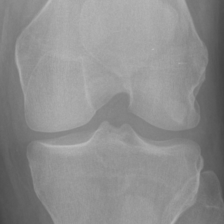
\includegraphics[width=1.7cm]{figs/KL0-sample.png} & 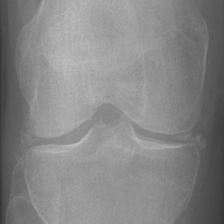
\includegraphics[width=1.7cm]{figs/KL1-sample.png} & 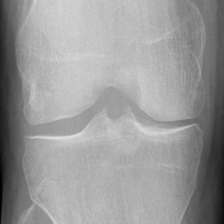
\includegraphics[width=1.7cm]{figs/KL2-sample.png} & 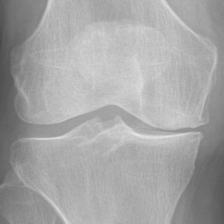
\includegraphics[width=1.7cm]{figs/KL3-sample.png} & 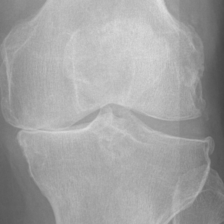
\includegraphics[width=1.7cm]{figs/KL4-sample.png} \\
        \hline
        \textbf{0 (saudável)} & \textbf{1 (duvidoso)} & \textbf{2 (mínimo)} & \textbf{3 (moderado)} & \textbf{4 (severo)} \\
        \hline
    \end{tabular}
    \caption{Escala de Kellgren/Lawrence para classificação da severidade de osteoartrite.}
    \label{tabela-kl}
\end{table}

\section{Rede Neural Convolucional (RNC)}\label{sec:rnc}

Uma rede neural artificial é um modelo computacional inspirado no cérebro humano \citep{McCulloch1943}, onde neurônios artificiais recebem um conjunto de entradas ponderadas, realizam uma soma dessas entradas e aplicam uma função de ativação para produzir uma saída. Essa estrutura permite que as redes neurais aprendam padrões complexos a partir de dados, tornando-as adequadas para tarefas de processamento de linguagem natural, visão computacional, entre outras aplicações.

Em 2006, \cite{Hinton2006} propuseram o uso de redes neurais artificiais com múltiplas camadas com o objetivo de melhorar a capacidade dos modelos, o que levou a um renascimento do interesse nessas redes e ao desenvolvimento de novas arquiteturas, como é o caso da rede neural convolucional (CNN, do inglês \textit{Convolutional Neural Network}).

As CNNs são modelos de aprendizado profundo projetados para processar dados com estrutura de grade, como imagens. Inspiradas na organização do córtex visual, CNNs são amplamente utilizadas em tarefas de visão computacional, como classificação de imagens, detecção de objetos e segmentação semântica.

A camada de convolução é o componente central das CNNs, responsável por extrair características locais dos dados de entrada. Essa camada utiliza filtros (ou \textit{kernels}), que são pequenas matrizes de pesos (por exemplo, 3x3 ou 5x5) aplicadas em toda a imagem de entrada para gerar um mapa de características (ou \textit{feature maps}), representando a presença dessas características em diferentes regiões da imagem.

Esses filtros são ajustados durante o treinamento da rede, permitindo que a CNN aprenda a detectar padrões relevantes, como bordas, texturas e formas. Conforme a rede avança pelas camadas, os filtros se tornam mais complexos e capazes de capturar características de alto nível, como objetos inteiros. Após as convoluções, é comum utilizar a função de ativação ReLU (\textit{Rectified Linear Unit}), que substitui valores negativos por zero e introduz não linearidades no modelo, permitindo que ele aprenda representações complexas.

Após as camadas de convolução, as CNNs geralmente incluem camadas de \textit{pooling} para reduzir a dimensionalidade dos \textit{feature maps}, enquanto preservam as características mais relevantes. O \textit{pooling} pode ser feito de várias maneiras, como \textit{max pooling} (onde o valor máximo de uma região é mantido) ou \textit{average pooling} (onde a média dos valores é calculada). Esse processo contribui para:

\begin{itemize}
    \item reduzir a quantidade de parâmetros e o custo computacional da rede.
    \item tornar a rede mais robusta a pequenas variações nos dados de entrada.
\end{itemize}

Após diversas camadas de convolução e \textit{pooling}, uma ou mais camadas totalmente conectadas (\textit{fully connected}) são adicionadas ao final da rede para combinar as características extraídas de camadas anteriores e realizar a tarefa de classificação. Cada neurônio dessas camadas está conectado a todos os valores da camada anterior, permitindo decisões baseadas em combinações globais das informações aprendidas. Em tarefas de classificação, a última camada totalmente conectada geralmente utiliza a função de ativação \textit{softmax}, que transforma as saídas em probabilidades.

Durante o treinamento, a CNN ajusta os pesos dos filtros por meio do algoritmo de retropropagação (\textit{backpropagation}), em que o erro de saída é retropropagado pela rede para atualizar os pesos e minimizar a função de perda. Esse processo é repetido por várias épocas, permitindo que a rede aprenda a reconhecer padrões complexos nos dados de entrada.

A \autoref{fig:cnn} ilustra uma rede neural convolucional composta por cinco camadas. O número de camadas, a disposição dessas camadas, o número e tamanho dos filtros, a forma de conexão entre as camadas, entre outros fatores, podem variar dependendo da arquitetura escolhida. Em seguida, serão aprensentadas algumas das arquiteturas populares de CNN que serão utilizadas neste trabalho.

\begin{figure}
    \centering
    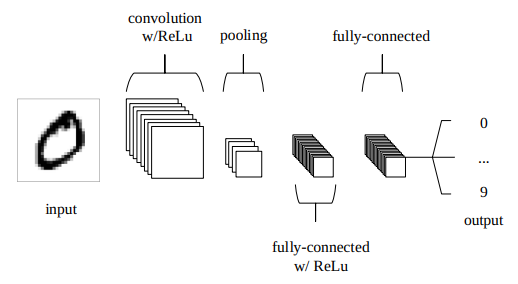
\includegraphics[width=0.5\linewidth]{figs/convolution-neural-network.png}
    \caption{Uma rede neural convolucional simples, composta por apenas cinco camadas. Fonte: \cite{Saxena2022}.}
    \label{fig:cnn}
\end{figure}

\subsubsection{Perceptron e Perceptron Multicamadas}

\subsubsubsection{Perceptron}

O tipo mais simples de rede neural é chamado de perceptron, que consiste num modelo linear baseado em um neurônio artificial capaz de fazer previsões binárias. Ele é muito similar à regressão linear, mas com a adição de uma função de ativação que transforma a saída em uma previsão binária \citep{James2000}. O perceptron pode ser definido pela seguinte fórmula:

\begin{equation}
    \hat{Y} = 
    \begin{cases}
        1 & \text{se } \sum_{i=1}^{n} w_i x_i > \theta \\
        0 & \text{caso contrário}
    \end{cases}
\end{equation}

onde $w_i$ são os pesos das variáveis preditoras $x_i$, $\theta$ é o limiar de ativação e $\hat{Y}$ é a previsão do modelo. Este algoritmo, também conhecido como perceptron de camada única, serve como base para as redes neurais artificiais e é usado para resolver problemas de classificação binária.

A \autoref{fig:perceptron} ilustra uma rede neural típica com uma camada de entrada, uma camada oculta e uma camada de saída. Este tipo de rede é capaz de modelar tanto problemas de classificação quanto de regressão, dependendo da função de ativação usada e o número de neurônios na camada de saída. Para um problema de classificação com K classes, existem K neuronios na camada de saída, cada um representando uma classe possível \citep{James2000}.

\begin{figure}
    \centering
    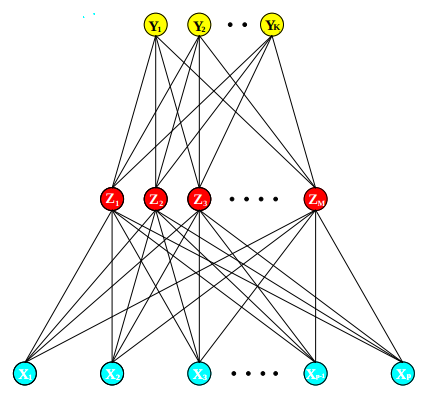
\includegraphics[width=0.5\linewidth]{figs/perceptron-network.png}
    \caption{Rede neural artificial com uma camada oculta. Fonte: \cite{James2000}.}
    \label{fig:perceptron}
\end{figure}

\subsubsubsection{Treinamento do Perceptron}

O treinamento do perceptron é feito através do algoritmo de aprendizado supervisionado, onde o modelo é ajustado iterativamente para minimizar a função de perda. O algoritmo mais comum para treinar o perceptron é o algoritmo de Rosenblatt \citep{Rosenblatt1958}, que busca encontrar um hiperplano que separe duas classes através da minimização da distância de pontos mal classificados em relação ao hiperplano.

A primeira etapa consiste em inicializar os pesos, normalmente com valores aleatórios baixos ou zero. É comum utilizar $w_i$ para representar o $i$-ésimo valor no vetor de pesos e $x_{j,i}$ para representar o valor da $i$-ésima variável preditora no $j$-ésimo valor no vetor de entrada de treinamento. Em seguida, é calculada a saída prevista $y_j$ para cada valor de entrada $x_j$ da seguinte forma:

\begin{equation}
    \begin{split}
        y_j(t) &= f[w(t) \cdot x_j] \\
        &= f[w_0(t) \cdot x_{j,0} + w_1(t) \cdot x_{j,1} + ... + w_n(t) \cdot x_{j,n}]
    \end{split}
\end{equation}

onde $f$ é a função de ativação e $w(t)$ é o vetor de pesos no tempo $t$. A saída prevista $y_j(t)$ é então comparada com o valor real $d_j$ para atualizar os pesos de acordo com a regra de aprendizado:

\begin{equation}
    w_i(t+1) = w_i(t) + \eta \cdot (d_j - y_j(t)) \cdot x_{j,i}
\end{equation}

onde $\eta$ é a taxa de aprendizado, que controla o tamanho do passo de atualização dos pesos. O algoritmo continua iterando sobre os dados de treinamento até que a função de perda $\frac{1}{s} \sum_{j=1}^{s} |d_j - y_j(t)|$ seja minimizada, onde $s$ é o número de observações no conjunto de treinamento, ou até que um critério de parada, como a convergência do erro, a acurácia do modelo ou o número máximo de iterações seja atingido.

\subsubsubsection{Perceptron Multicamadas}

Ao adicionar múltiplas camadas de neurônios entre a entrada e a saída, forma-se o que se denomina perceptron multicamadas (MLP – \textit{Multilayer Perceptron}), geralmente composto por uma camada de entrada, uma ou mais camadas ocultas — responsáveis pelo processo de aprendizado — e uma camada de saída \citep{Sarker2021}. A \autoref{fig:multilayer-perceptron} apresenta uma arquitetura típica de um MLP.

Quando a rede neural é expandida com várias camadas ocultas, ela passa a ser chamada de rede neural profunda (\textit{Deep Neural Network}), capaz de aprender representações hierárquicas, mais complexas e abstratas dos dados \citep{AurlienGron2019}. Esse tipo de arquitetura permite a resolução de problemas altamente não lineares e desafiadores, frequentemente presentes em tarefas como visão computacional, processamento de linguagem natural e reconhecimento de voz.

\begin{figure}[h]
    \centering
    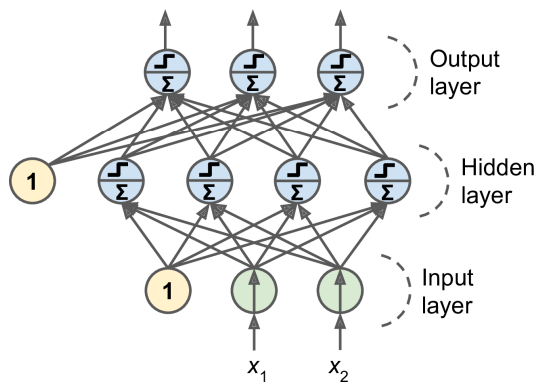
\includegraphics[width=\linewidth]{figs/multilayer-perceptron.png}
    \caption{Arquitetura de uma rede perceptron multicamadas com duas entradas, uma camada oculta de quatro neurônios e três neurônios de saída (os neurônios de viés são mostrados, mas normalmente estão implícitos). Fonte: \cite{AurlienGron2019}.}
    \label{fig:multilayer-perceptron}
\end{figure}

\subsubsection{Funções de Ativação}

As funções de ativação desempenham um papel fundamental nas redes neurais artificiais, pois são responsáveis por introduzir não linearidade no modelo e melhorar a convergência da rede \citep{Dubey2022}. Sem elas, independentemente do número de camadas ocultas adicionadas, a rede se comportaria como um modelo linear, incapaz de aprender e representar padrões complexos e não lineares dos dados.

Matematicamente, uma função de ativação $f$ transforma a saída $z$ de um neurônio em uma nova saída $f(z)$, que será propagada para as camadas seguintes da rede. Algumas das funções de ativação mais comuns incluem:

\begin{itemize}
    \item \textbf{Sigmoide}: é uma função limitada e diferenciável, que tem exatamente um ponto de inflexão. Devido a sua característica de limitar valores em um intervalo definido, ela é chamada de função de compressão (ou \textit{squashing function} do inglês) \citep{lederer2021activation}. A função sigmoide logística, também conhecida como função logística, é definida como:
    
    \[
    f(z) = \sigma(z) = \frac{1}{1 + e^{-z}}
    \]
    
    Essa função mapeia os valores de entrada para o intervalo $(0, 1)$, o que a torna útil para modelar probabilidades. Por isso, a função sigmoide é frequentemente utilizada em problemas de classificação binária, onde a saída é interpretada como uma probabilidade \citep{nwankpa2018activation}.

    Apesar de ser historicamente importante na teoria e prática de redes neurais, a função sigmoide sofre com o problema do \textit{desvanecimento do gradiente} (\textit{vanishing gradient}), onde os gradientes se tornam muito pequenos durante o treinamento, dificultando a atualização dos pesos e levando a um aprendizado lento ou estagnado, especialmente em redes profundas \citep{Dubey2022}.

    \item \textbf{Tangente Hiperbólica (tanh)}: é uma função de ativação semelhante à sigmoide, mas com a vantagem de ser centrada em zero, o que pode contribuir para a convergência do modelo, além de ter uma saída mais ampla, variando entre -1 e 1 \citep{nwankpa2018activation}. A função tangente hiperbólica é definida como:
    
    \[
    f(z) = \tanh(z) = \frac{e^{z} - e^{-z}}{e^{z} + e^{-z}}
    \]
    
    A função tanh também sofre com o problema do desvanecimento do gradiente, mas em menor grau do que a sigmoide \citep{Dubey2022}. Outra condição importante a ser considerada é que a função tanh pode produzir ``neurônios mortos'' quando a entrada é muito grande ou muito pequena, resultando em gradientes nulos e impedindo a atualização dos pesos \citep{nwankpa2018activation}.

    \item \textbf{ReLU (Rectified Linear Unit)}: atualmente uma das funções mais utilizadas em aplicações de aprendizado profundo, a ReLU é uma função de ativação mais rápida e eficiente do que a sigmoide e a tangente hiperbólica \citep{Nair2010}. De forma simples, a ReLU é uma função linear que retorna o valor de entrada se ele for maior que zero, e zero caso contrário, definida como:
    
    \[
    f(z) = \max(0, z) =
    \begin{cases}
        z, & \text{se } z > 0 \\
        0, & \text{caso contrário}
    \end{cases}
    \]

    Ela resolve parcialmente o problema do desvanecimento do gradiente, mas pode levar à inatividade de neurônios quando $z < 0$ \citep{Dubey2022}. Apesar disso, a ReLU é amplamente utilizada em redes neurais profundas devido à sua simplicidade e eficiência computacional.

    \item \textbf{Leaky ReLU}: é uma variação da ReLU que introduz uma pequena inclinação para valores negativos, evitando que os neurônios fiquem permanentemente inativos durante o processo de treinamento \citep{Maas2013}. O parâmetro $\alpha$ controla a inclinação da função para valores negativos, evitando que os gradientes sejam zero \citep{nwankpa2018activation}. A Leaky ReLU é definida como:
    
    \[
    f(z) = \alpha z + z =
    \begin{cases}
    z, & \text{se } z > 0 \\
    \alpha z, & \text{caso contrário}
    \end{cases}
    \]

    onde $\alpha$ é um pequeno valor positivo, tipicamente 0{,}01.

    \item \textbf{Softmax}: é uma função de ativação usada para computar a distribuição de probabilidade de um vetor de valores reais, onde a soma das saídas é igual a 1 \citep{nwankpa2018activation}. A função softmax é definida como:
    
    \[
    f(z_i) = \frac{e^{z_i}}{\sum_{j=1}^{K} e^{z_j}}, \quad \text{para } i = 1, 2, \dots, K
    \]

    onde $K$ é o número total de classes.

    A função softmax é frequentemente utilizada na camada de saída de redes neurais para problemas de classificação multiclasse, onde cada neurônio na camada de saída representa uma classe e a saída da função softmax é interpretada como a probabilidade de cada classe \citep{nwankpa2018activation}.

\end{itemize}

\subsubsection{Algoritmo de Retropropagação}

Quando se trata de aprendizado supervisionado em redes neurais, o algoritmo de retropropagação (ou \textit{backpropagation} em inglês) é um dos métodos mais utilizados para treinar modelos de redes neurais artificiais, especialmente em redes multicamadas \citep{Sarker2021}. Este algoritmo funciona ajustando os pesos dos neurônios de maneira a minimizar a função de perda através do cálculo do gradiente do erro da rede em relação aos pesos \citep{AurlienGron2019}.

O algoritmo consiste em duas etapas principais: a fase de propagação para frente e a fase de retropropagação. Na fase de propagação para frente, os dados de entrada são transmitidos através da rede, camada por camada, até chegar à camada de saída. Durante essa fase, cada neurônio calcula sua saída com base nas entradas recebidas e nos pesos associados, aplicando a função de ativação correspondente (Sigmoide, ReLU, etc.). Por exemplo, para um neurônio $k$, sua saída $h_k$ é dada por $h_k = f(a_k)$, onde $a_k = \sum_{j} h_j W_{jk}$, $f$ é a função de ativação e $W_{jk}$ é o peso associado à conexão entre o neurônio $j$ e o neurônio $k$ (\autoref{forward-pass}). A saída final da rede é então comparada com o valor real usando uma função de perda (MSE, entropia cruzada, etc.), que quantifica o erro da previsão. Por exemplo, para um neurônio $l$ da camada de saída, o erro é calculado usando a saída prevista $y_l$ e o valor real $t_l$ \citep{Lillicrap2020}.

\begin{figure}[h]
    \centering
    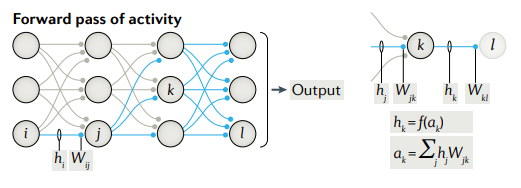
\includegraphics[width=\linewidth]{figs/forward-pass.png}
    \caption{Propagação para frente. Fonte: \cite{Lillicrap2020}.}
    \label{forward-pass}
\end{figure}

Na fase de retropropagação (), o erro calculado na camada de saída é propagado de volta através da rede, ajustando os pesos de cada neurônio com base na contribuição para o erro. Isso é feito usando a regra da cadeia, que permite calcular o gradiente do erro em relação aos pesos \citep{AurlienGron2019}. A forma mais simples de usar o gradiente é mudar cada peso $W_{ij}$ na direção do gradiente negativo, ou seja:

\begin{equation}
    \Delta W_{ij} = -\eta \frac{\partial E}{\partial W_{ij}} = -\eta h_i \delta_j
\end{equation}

onde $\eta$ é a taxa de aprendizado, $E$ é a função de perda, e $\delta_j = e_j f'(a_j) = (\sum_k \delta_k W_{jk}) f'(a_j)$ é o erro do neurônio $j$ na camada oculta \citep{Lillicrap2020}. A retropropagação continua até que todos os pesos da rede sejam atualizados, minimizando assim a função de perda. Esse processo é repetido para várias iterações ou épocas, até que o modelo converja para um conjunto de pesos que minimizam o erro.

\begin{figure}[h]
    \centering
    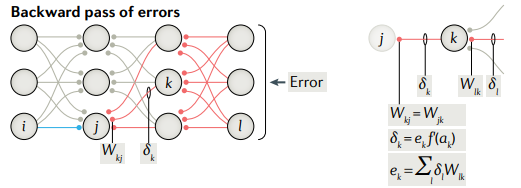
\includegraphics[width=\linewidth]{figs/backward-pass.png}
    \caption{Retropropagação. Fonte: \cite{Lillicrap2020}.}
    \label{backward-pass}
\end{figure}

\subsubsection{Otimização de Redes Neurais}

A otimização de redes neurais é um aspecto crucial no treinamento de modelos de aprendizado profundo, pois envolve a escolha de algoritmos e técnicas que permitem ajustar os pesos da rede para minimizar a função de perda.

Um dos algoritmos mais populares para otimização de redes neurais é o \textit{Gradient Descent} \citep{Ruder2017}. No entanto, existem outros algoritmos, cada um com suas próprias características e vantagens, que podem ser adequados para diferentes tipos de problemas e arquiteturas de redes neurais, como por exemplo o \textit{Stochastic Gradient Descent} (SGD), \textit{Momentum}, \textit{Nesterov Accelerated Gradient} (NAG), Adagrad, Adadelta, RMSprop e Adam.

Para tarefas de visão computacional, \cite{Kingma2015} mostraram que o Adam é um dos algoritmos de otimização mais eficazes em redes neurais convolucionais. Testes no conjunto de dados MNIST mostraram que o Adam convergiu mais rapidamente e alcançou melhores resultados em comparação com outros algoritmos, como SGD e Adagrad.

\section{Visão Computacional}\label{sec:visao-computacional}

A visão computacional é um campo da inteligência artificial (IA) e da ciência da computação (\autoref{definicao-cv}) que estuda como as máquinas podem adquirir, processar, analisar e compreender imagens e vídeos do mundo real, com o objetivo de produzir representações visuais ou descrever o conteúdo visual de forma automática \cite{huggingface2024}.

\begin{figure}[h]
    \centering
    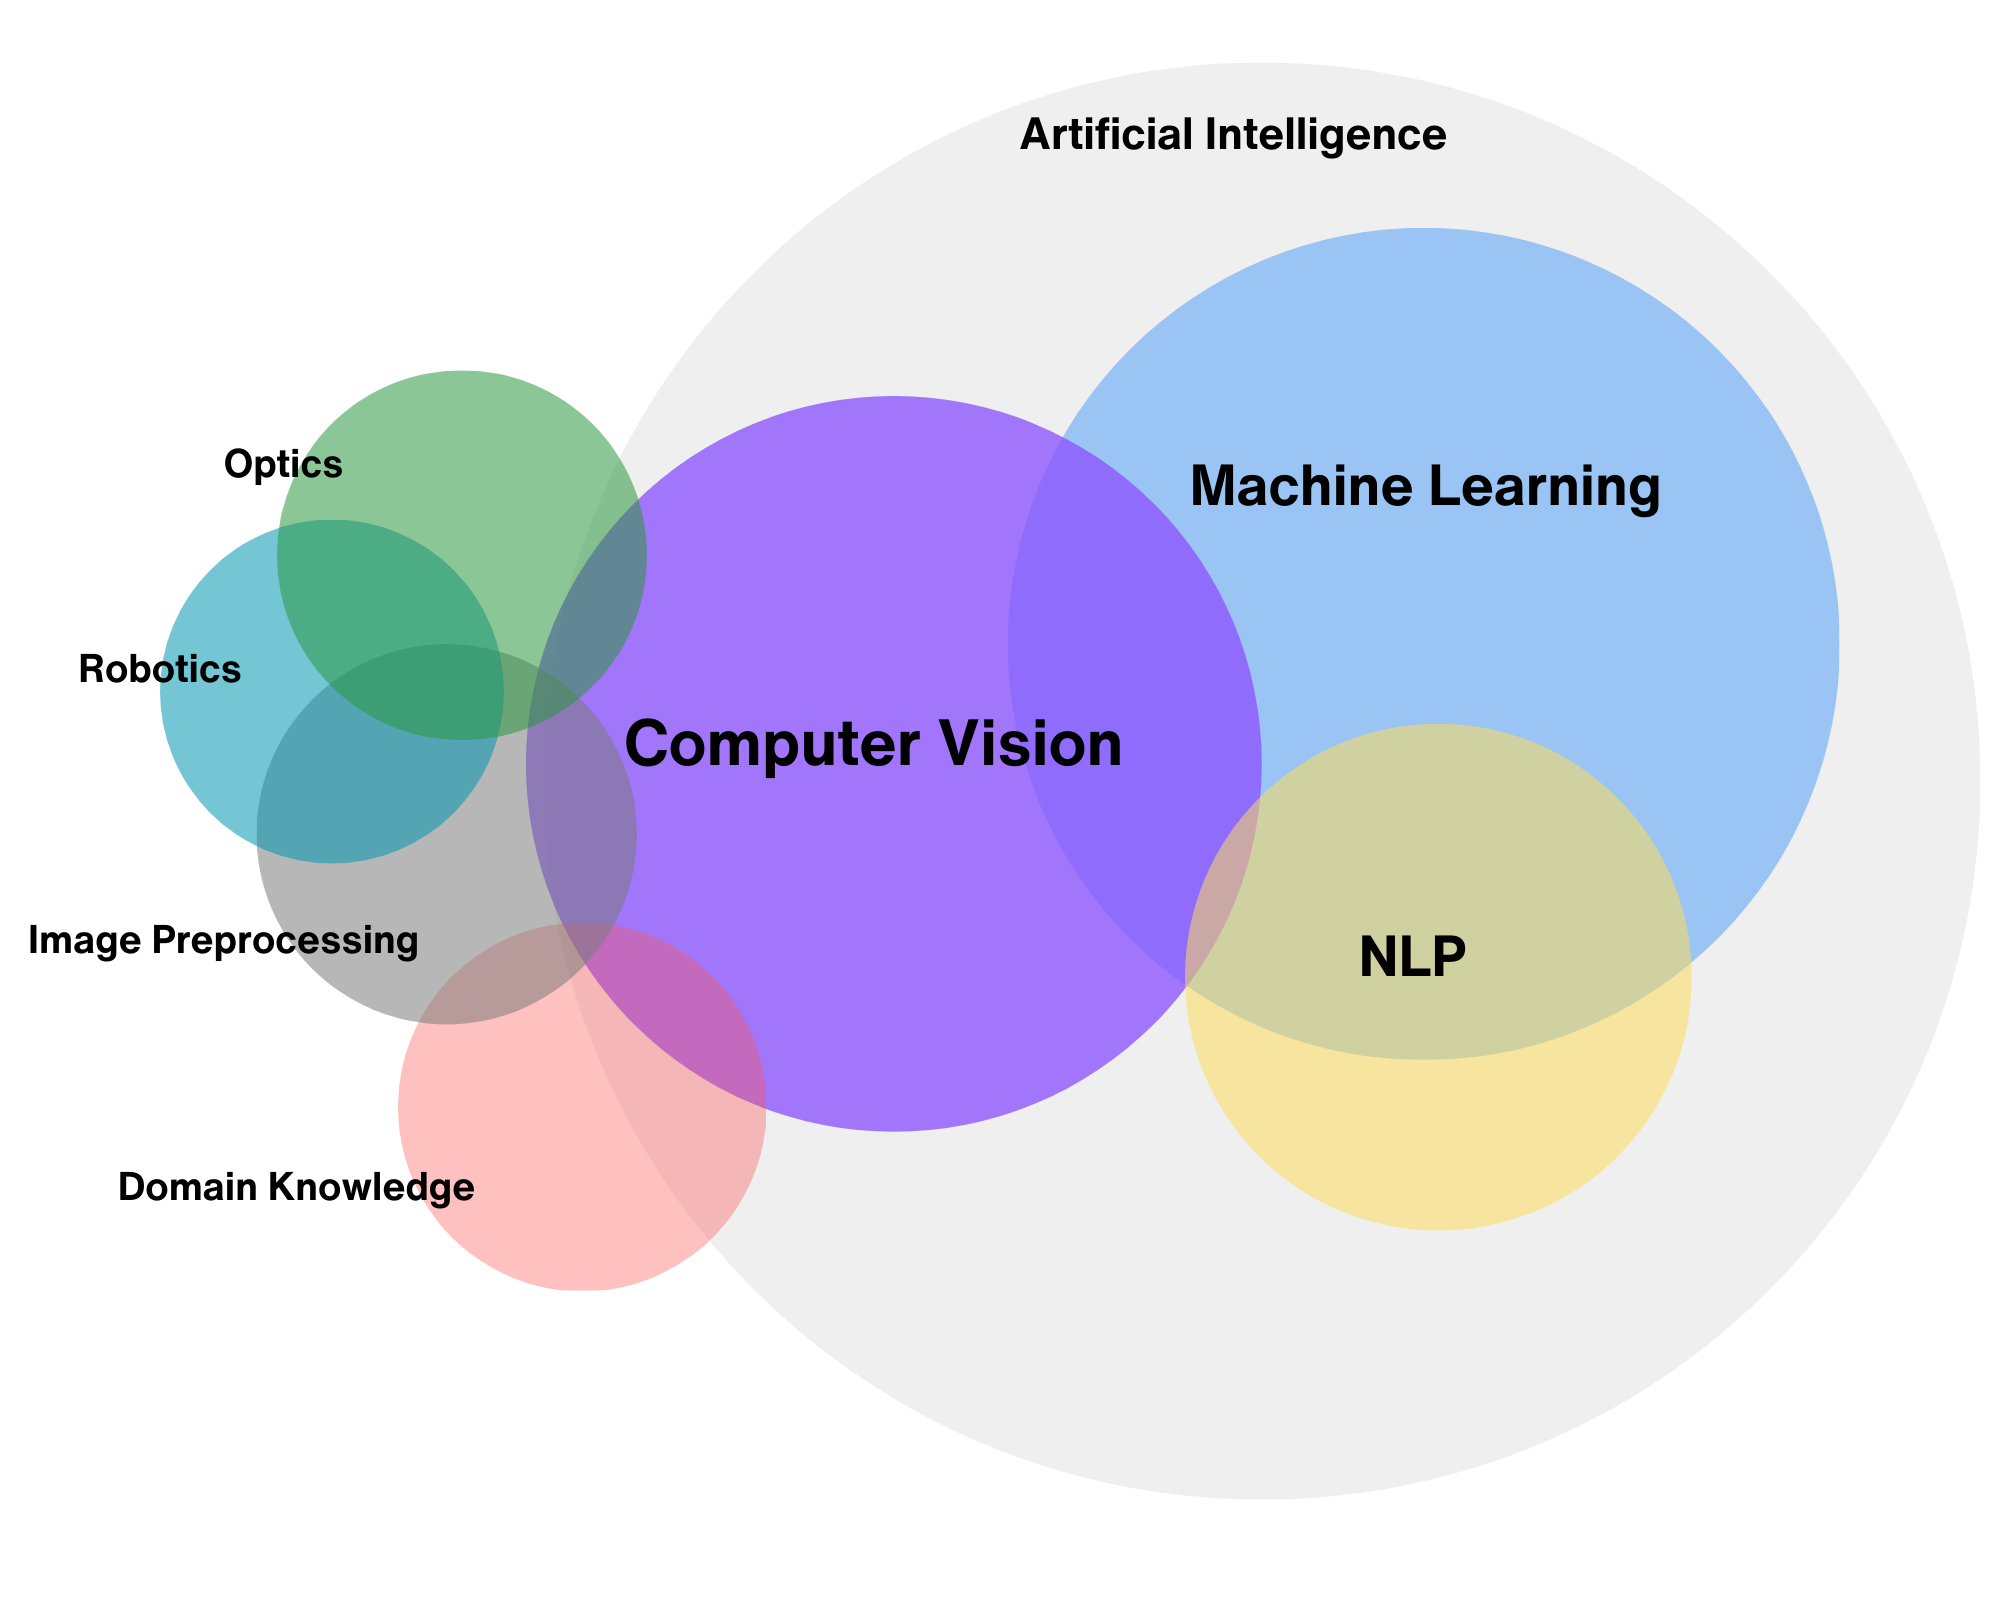
\includegraphics[width=\linewidth]{figs/CV_in_defintiion.png}
    \caption{Definição de visão computacional. Fonte: \cite{huggingface2024}.}
    \label{definicao-cv}
\end{figure}

Essa tecnologia tem se beneficiado de avanços significativos das últimas décadas, incluindo o desenvolvimento e aperfeiçoamento de algoritmos de aprendizado profundo, que permitem a extração de características complexas e abstratas de imagens e vídeos, o aumento da capacidade computacional com o uso de GPUs (Graphics Processing Units), e o desenvolvimento de grandes conjuntos de dados, como o ImageNet, que contém milhões de imagens rotuladas em centenas de categorias \cite{Esteva2021}.

O aprendizado profundo revolucionou a forma como sistemas computacionais processam dados brutos. Tradicionalmente, a construção de modelos exigia conhecimento especializado para extrair manualmente características relevantes dos dados, como bordas, texturas e formas. Enquanto isso, o aprendizado profundo permite que redes neurais descubram automaticamente essas representações em vários níveis de abstração. Esse avanço tem levado a conquistas notáveis em diversas áreas, como reconhecimento de fala, processamento de linguagem natural (PLN) e visão computacional [https://www.cs.toronto.edu/~hinton/absps/NatureDeepReview.pdf].

Em 1963, Larry Roberts, um dos pioneiros da visão computacional, propôs métodos capazes de compreender objetos em 3D a partir de imagens 2D, representando o marco inicial da área [Machine Perception of Thre Dimensional Solids]. Na próxima década, nos anos 1970 e 1980, pesquisadores desenvolveram algoritmos para detectar bordas e cantos em imagens, modelagem poliédrica e não poliédrica, representação de objetos como interconexões de estruturas menores, fluxo óptico e estimativa de movimento [computer vision: algorithms and applications]. Além disso, a década de 1980 foi marcada pela publicação do artigo "Learning representations by back-propagating errors" de David Rumelhart, Geoffrey Hinton e Ronald Williams, que introduziu o algoritmo de retropropagação, que é amplamente utilizado em modelos de aprendizado profundo até hoje [NatureDeepReview, Learning representations by back-propagating errors].

No entanto, foi apenas na decada de 2010 que o aprendizado profundo se tornou popular, com o desenvolvimento de arquiteturas de redes neurais profundas, como as redes neurais convolucionais (CNNs) e as redes neurais recorrentes (RNNs), amplamente adotadas pela comunidade de visão computacional [https://www.cs.toronto.edu/~hinton/absps/NatureDeepReview.pdf]. Em 2012, a equipe de Geoffrey Hinton, chamada de Super Vision, venceu a competição ImageNet Large Scale Visual Recognition Challenge (ILSVRC) com a rede neural convolucional AlexNet, que alcançou resultados significativamente melhores do que os métodos tradicionais de visão computacional em tarefas de classificação e detecção de objetos em imagens [https://arxiv.org/pdf/1409.0575]. Esse avanço marcou a início da era do aprendizado profundo na visão computacional, permitindo a crição de modelos mais sofisticados e precisos, capazes de superar a capacidade humana em tarefas visuais.

Paralelamente, houve uma evolução significativa em hardware computacional, com o desenvolvimento de GPUs, que permitiu treinar modelos de aprendizado profundo em grandes conjuntos de dados de forma mais rápida e eficiente. As GPUs, inicialmente projetadas para renderização de gráficos em jogos e aplicações de design, foram adaptadas para acelerar cálculos matriciais e aplicações computacionalmente intensivas, incluindo o treinamento de redes neurais profundas, devido à sua capacidade de processar informação em paralelo [High performance convolutional neural networks for document processing, Forecasting GPU Performance for Deep Learning Training and Inference]. Em 2009, a equipe de Andrew Ng, da Universidade de Stanford, demonstrou que o uso de GPUs acelerou o treinamento de redes neurais profundas em 70 vezes em comparação com CPUs multi-core, o que permitiu a criação de modelos mais complexos em menos tempo [Large-scale Deep Unsupervised Learning using Graphics Processors]. A partir de então, GPUs se tornaram uma ferramenta essencial para pesquisadores e instituições que trabalham com aprendizado profundo, trazendo mais agilidade e eficiência para o treinamento de modelos.

Apesar dos avanços em algoritmos de aprendizado profundo e hardware computacional, a visão computacional ainda enfrentava desafios quanto à falta de grandes conjuntos de dados rotulados para treinar os modelos de visão computacional. No entanto, em 2009 foi introduzido o ImageNet, um conjunto de dados com milhões de imagens em centenas de categorias, construído sobre a base de dados WordNet, que contém sinônimos e relações semânticas entre palavras. Com isso, o ImageNet se tornou o maior e mais diverso conjunto de dados de imagens disponível na época [ImageNet: A Large-Scale Hierarchical Image Database]. Mais tarde, em 2012, o ImageNet serviu como base para o ImageNet Large Scale Visual Recognition Challenge (ILSVRC), uma competição anual que avalia algoritmos de classificação e detecção de objetos em larga escala. O desafio foi marcado pela vitória da equipe de Geoffrey Hinton, onde propuseram a rede neural convolucional profunda chamada AlexNet capaz de alcançar altas taxas de acurácia e redução significativa na taxa de erro, marcando assim o início da era do aprendizado profundo e solidificando o papel do ImageNet como catalisador para inovações subsequentes na área [ImageNet Large Scale Visual Recognition Challenge].

[tecnicas da visao computacional]

[aplicacoes gerais]

\section{Visão Computacional na Saúde}\label{sec:visao-computacional-saude}

No setor da saúde, a visão computacional tem desempenhado um papel crucial na automação de tarefas clínicas, diagnóstico de doenças, monitoramento de pacientes e tratamentos médicos. A análise de imagens médicas, como radiografias, tomografias, ressonâncias magnéticas e ultrassonografias, é uma das principais aplicações da visão computacional na saúde. A partir dessas imagens, é possível detectar e classificar patologias, monitorar o progresso de doenças, avaliar a eficácia de tratamentos e até mesmo recomendar tratamentos personalizados para pacientes. Além disso, a visão computacional também tem sido utilizada para automatizar tarefas clínicas, como a identificação de pacientes, a análise de exames laboratoriais e a triagem de pacientes em hospitais e clínicas \cite{JAVAID2024792}.

Na área da saúde, a visão computacional tem sido muito utilizada para melhorar a acurácia de diagnósticos, automatização de tarefas clínicas e tratamentos médicos. Ao analisar imagens médicas, como radiografias, tomografias, ressonâncias magnéticas e ultrassonografias, a máquina pode detectar e classificar patologias com maior precisão e rapidez do que um médico humano. Além disso, a visão computacional pode ser utilizada para monitorar o progresso de doenças, monitorar a eficácia de tratamentos e até mesmo recomendar tratamentos personalizados para pacientes \cite{JAVAID2024792}.

\section{Aprendizado Profundo}\label{sec:aprendizado-profundo}

O uso de modelos de aprendizado profundo baseados em redes neurais convolucionais (RNCs) tem ganhado espaço em tarefas de visão computacional. Aprendizado por transferência também é amplamente utilizado para reduzir o uso de recursos computacionais para tarefas que já são executadas por modelos existentes, como as redes residuais (ResNet), Visual Geometry Group (VGG) e as redes densamente conectadas (DenseNet) \cite{Tariq2023}. Enquanto o uso de RNCs tem se mostrado útil em soluções de detecção em imagens médicas, a operação de convolução limita o relacionamento entre pixels distantes numa imagem. Para tanto, a habilidade de codificar dependências de longo alcance tem sido possível graças às arquiteturas de aprendizado profundas baseadas em atenção, como o Vision Transformer (ViT). Tais modelos de ViT têm sido empregados para várias tarefas, incluindo classificação e detecção de objetos \cite{Shamshad2023}.

% \section{Transferência de Aprendizado e Ajuste Fino}\label{sec:ajuste-fino}

\section{Avaliação e métricas de desempenho} \label{sec:avaliacao-metricas}

\subsection{Predição Conformal}

A predição conformal é uma técnica que fornece intervalos de confiança para previsões feitas por qualquer modelo de aprendizado de máquina. Dada uma probabilidade de erro $\epsilon$, a predição conformal gera um conjunto de possíveis rótulos para um novo exemplo $y$, incluindo o rótulo $\hat{y}$ fornecido pelo modelo e, geralmente, o rótulo verdadeiro com probabilidade de pelo menos $1 - \epsilon$ \citep{angelopoulos2021gentle}.

Suponha um modelo classificador $\hat{f}$ e um conjunto de imagens classificadas em uma das $K$ classes possíveis. Para cada imagem, o modelo atribui uma probabilidade $\hat{f}(x) \in [0,1]^K$ para cada classe, normalmente usando a função \textit{softmax}. Em seguida, um conjunto de imagens de calibração é utilizado para encontrar um limiar de confiança $\hat{q}$, que é o valor mínimo de probabilidade para considerar uma classe como possível. A etapa de calibração é feita da seguinte forma:

\begin{enumerate}
    \item Para cada par ($X_i$,$Y_i$) de imagem do conjunto de calibração, calcula-se a pontuação de conformidade $s_i = 1 - \hat{f}(X_i)_{Y_i}$
    \item Ordena-se as pontuações de conformidade em ordem crescente: $s_1 \leq s_2 \leq ... \leq s_n$
    \item Define-se o limiar de confiança $\hat{q}$ como o quantil ${\lceil (n+1)(1-\epsilon) \rceil}/n$ sobre $s_1, ... s_n$, onde $\lceil \cdot \rceil$ é a função teto.
\end{enumerate}

Dessa forma, dada uma nova imagem de teste $X_{\text{test}}$, a predição conformal gera um conjunto de rótulos possíveis $C(X_{\text{test}}) = \lbrace y:s(X_{\text{test}},y) \leq \hat{q} \rbrace$, que inclui todas as classes cujo valor \textit{softmax} é maior ou igual ao limiar de confiança $\hat{q}$.

Como uma extensão da predição conformal, \cite{angelopoulos2021gentle} introduziram um método para para gerar intervalos de confiança, chamado de \textit{adaptive prediction sets} (APS). Esse método é baseado na ideia de que, em vez de gerar um conjunto de rótulos com o menor tamanho médio, o modelo pode gerar um conjunto adaptativo de rótulos, que se ajusta dinamicamente ao nível de incerteza do modelo.

Seguindo o APS, o conjunto de rótulos $\lbrace y: s(x,y) \leq \hat{q} \rbrace$ é definido da seguinte forma:

\begin{equation}
    C(x) = \lbrace \pi_1(x), ..., \pi_k(x) \rbrace \text{, onde } k = \sup \Bigg\lbrace k' : \sum_{j=1}^{k'} \hat{f}(x)_{\pi_j(x)} < \hat{q} \Bigg\rbrace + 1
\end{equation}

A predição conformal tem sido aplicada em diversas áreas, incluindo ciência forense, biometria e medicina, onde o objetivo é fornecer previsões mais confiáveis sobre a saída do modelo \citep{Fontana2023}. Por exemplo, \cite{Pereira2020} utilizaram a predição conformal para prever o intervalo de confiança da probabilidade de que pacientes com comprometimento cognitivo leve evoluam para demência.